\section{Proposed Research and Timeline}
To start the research for my PhD thesis I seek to explore phonon softening and charge ordering phenomena in \ts.
Former work of the Siwick Group on \ts\space shows that photoexciting carriers into the 3d conduction band leads to a stiffening of transverse phonons at the M points\cite{otto2021}.
The coupling between free carriers and phonons, however, is not enhanced, which is in striking contrast to the behavior observed in graphite\cite{stern2018}.
Both experiment were conducted at room temperature.
The \ac{CDW} phase with its excitonic ground state should be fragile against large densities of free charge carriers due to screening effects.
It would be interesting to investigate the dynamics of the excitonic ground state decaying upon photo-excitation and its subsequent reformation upon cooling, while systematically varying the pump-fluence.
Hedayat et al. published an article with a similar approach using time- and angle-resolved photoenmission spectroscopy and time-resolved reflectivity measurements\cite{hedayat2019}.
They observe a transient gain in the spectral intensity of the valence band at the $\Gamma$ point at 80\,K, whereas there is no gain to be seen at 300\,K.
It is argued that the intensity gain arises from the valence band at the M point unfolding to $\Gamma$, which is an indicator of the breaking of excitons and a distortion of the \ac{CDW}.
Their reflectivity measurements unveil two phonon modes that strongly couple to the excitonic ground state, which are referred to as \acp{SCP}.
A model is derived that links hot carriers and \acp{SCP}, via exciton formation and annihilation.
An exciton formed by two hot carriers will create an \ac{SCP}, whereas an \ac{SCP} absorbed by an hot carriers creates forms an exciton.
A large population of \ac{SCP} will bottleneck the excitonic ground state recovery.
\Acp{SCP} may also decay into heat via anharmonic coupling.
The bottleneck preventing rapid recovery is determined by the ratio of the exciton annihilation events and the anharmonic coupling events.
In this model the relaxation to the ground state is limited by anharmonic coupling.
For fluences above 0.1\,$\frac{\mathrm{mJ}}{\mathrm{cm^2}}$ the bottleneck emerges as the exciton annihilation becomes dominant.

\begin{figure}[!t]
	\begin{minipage}{0.5\columnwidth}
		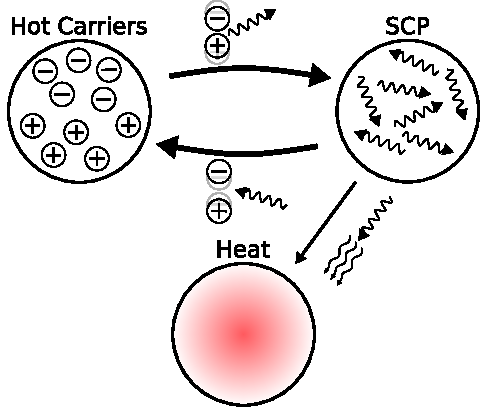
\includegraphics[width=\columnwidth]{figs/phonon_bottleneck.pdf}
	\end{minipage}
	\hspace{0.04\columnwidth}
	\begin{minipage}{0.45\columnwidth}
		\caption{Schematic of the phonon bottleneck model with three interactions and three reservoirs, namely hot carriers, strong coupling phonons (SCPs) and heat. Free carriers can form an exciton while emmiting a SCP. Vice versa phonons can be absorbed by an exciton, creating a pair of hot carriers. The last transition describes anharmonic decay of SCPs into different phonon populations that are regarded to as heat.}
		\label{fig:model}
	\end{minipage}
\end{figure}

I propose that our experiment is capable to retrieve considarably more information from the phononic processes discussed in this model.
Simulations of the low temperature phase and \ac{UEDS} measurements will allow the determination of both \ac{SCP} modes populations.
One of the modes is associated to the \ac{PLD} and not present in the high temperature phase.
The second modes origin is still under discussion; it is energetically similar to the $A_{1g}$ mode of the normal phase\cite{holy1977}.
Disentangling both contributions can give interesting insights for the formation of the low temperature phase.

From an experimental point of view, at this point in time it is not possible to control the temperature of the sample.
The installation of a closed-cycle cryostat is currently ongoing at will allow access to sample temperatures of 4-800\,K.
In addition to that, the machine is subject to more upgrades.
First, we have reduced the physical length of the instrument, reducing the influence of space-charge effects of the electron bunch on the time resolution.
Second, a Faraday cup has been designed and machined and is ready for installation to measure number of electrons in the bunches.
This allows for further characterization and better control of the instrument.
Third, a new detector camera (Dectris Quadro \cite{dectris2022}) has been installed and implemented in the laboratory software system.
Instead of a conventional CCD chip coupled to a scintillator, the detector is a \emph{hybrid pixel detector} consisting of bare silicon pixels that can directly count incoming electrons.
Signal-to-noise ratio dramatically improved and the read-out electronics are fast enough to capture diffraction images of every single electron bunch.
In addition to that the high dynamic range makes the use of a beam stop obsolete; the full diffraction pattern can be captured and analyzed.
Finally, the Dectris Quadro is much less sensitive to scattered light from pump and probe beam, which helps to produce less distorted diffraction images.

The previous work performed on \ts\space in the Siwick Group combined with new capabilities of the modified experimental setup provide a solid base to investigate the \ac{CDW} phase transition in new ways.
At a later stage it could be promising to not only probe the $\Gamma\mathrm{MK}$ plane of the \ac{BZ}, but also access the L point.
Earlier this year a \ac{UED} study accessing the $\overline{\mathrm{ML}}$ path revealed the lift of correlation of the \ac{CDW} along the c-axis upon photoexcitation.
A dimensional crossover towards 2$\times$2 \ac{CDW} is proposed\cite{cheng2022}.
The problem of forfeiting time resolution has been overcome by other groups encountering similar issues in time-resolved diffraction experiments.
The idea is to compensate the velocity mismatch of pump and probe pulse by tilting the optical pump pulse.
This leads to synchronous time delay of pump and probe event across the whole sample area\cite{baum2006,zhou2013}.
While conducting experiments on tilted samples without introducing a tilt to wave front of the pump pulse is possible, setting up a pulse front tilting stage would enhance the data quality considerably.

Another particularly interesting feature of \ts\space is, that upon intercalation with copper it will become superconducting below a critical temperature of 4.15\,K\cite{morosan2006}.
Since superconductivity is a phenomenon caused by the cooperative behavior of electrons coupled by phonons, these effects seem to be related to the \ac{CDW}/\ac{PLD} formation.
As of right now I don't explicitly plan to investigate Cu-intercalated samples, but I am certainly aware of these aspects.

\subsection*{Timeline}
My goal is to submit my PhD thesis at the end of 2025, which would correspond to an overall duration of four years.
The next six months will be primarily devoted to machine upgrades, data collection and simulations on the low-temperature phase of \ts.
With the temperature controllable sample stage being ready in summer, a comprehensive dataset of the decay and formation dynamics of the low temperature phase of \ts may be collected.
In the meantime I am working on the calculation on the one-phonon structure factor of the low temperature phase.
The 2$\times$2$\times$2 lattice reconstruction leads to an 8-fold increase in atoms per unit cell, which is making these simulations particularly challenging.
Data analysis and preparation of a manuscript should follow in the beginning of 2023.
After the first run of experiments I plan to further extend the machine capabilities and access the L points of the \ac{BZ}.
A positioning system to tilt the sample stage is already available; the setup of a pulse-front tilting optical stage will require rather simple optical equipment, namely a grating, some mirrors, lenses and positioning tools.
With these extensions a new degree of freedom can be probed.
Depending on the results of the first experiment run, I might want to dig deeper into the mechanisms studied in the first run, or even look into related material systems.
An interesting approach could be to repeat afformentioned experiments on monolayers of \ts, since the contribution of lattice and excitonic degrees of freedom to the \ac{CDW} drasticlly changes when going from bulk to monolayer systems.
Tristan Britt has recently shown that our machnine is capable of collecting diffraction patterns with meaningful signal-to-noise ratio from monolayer MoS\textsubscript{2} samples.